\documentclass[conference]{IEEEtran}
\IEEEoverridecommandlockouts
% The preceding line is only needed to identify funding in the first footnote.
% If that is unneeded, please comment it out.
\usepackage{amsmath,amssymb,amsfonts}
\usepackage{algorithmic}
\usepackage{graphicx}
\usepackage{textcomp}
\usepackage{xcolor}
\usepackage{natbib}
\usepackage{graphicx}

\usepackage{todonotes}
\newcommand{\cit}[1][]{\todo[tickmarkheight=0.2cm]{cit #1}}

\def\BibTeX{{\rm B\kern-.05em{\sc i\kern-.025em b}\kern-.08em
    T\kern-.1667em\lower.7ex\hbox{E}\kern-.125emX}}
\begin{document}

\title{Measuring fidelity in AI explanations:\\an open problem of the XAI field}

\author{\IEEEauthorblockN{Alvise de' Faveri Tron}
    \IEEEauthorblockA{\textit{Politecnico di Milano} \\
        alvise.defaveri@mail.polimi.it}}

\maketitle

\begin{abstract}
    Artificial Intelligence is known to suffer from interpretability problems:
    it is often hard for humans to explain why an AI took a particular decision
    or to understand what is the general logic behind its behavior. This is a
    serious ethical and technical barrier for the progress of AI, since this
    opaqueness has led, in some cases, to the realization of AI algorithms that
    behave in weird, unfair or dangerous ways. XAI (short for eXplainable AI) is
    a new research field that aims at solving this problem by providing some
    kind of explanation interface between humans and AI algorithms. However, at
    the moment, solutions in this field are being proposed without a widely
    accepted, common definition of \textit{interpretability}. A common metric
    used for evaluating the interpretability of XAI solutions is complexity, for
    example the number of leafs in a decision tree: this is clearly not enough,
    since many other aspects, such as the usefulness and the preciseness of the
    explanations, are not taken into account. In particular, a commonly
    overlooked feature of explanations is \textit{fidelity}, i.e. how closely
    does the explanation resemble the original system. This feature is generally
    opposed to simplicity, and the fact that many studies fail to explicitly
    measure this tradeoff leads to the following questions: how can we trust an
    explanation interface if we can't measure how accurately it represents the
    original AI system? Can inaccurate explanations introduce biases themselves
    by hiding or distorting aspects of the original model? If this is the case,
    isn't XAI introducing new trust issues instead of solving the existing ones
    that are inherent to AI?
\end{abstract}

% 1. AI suffers from interpretability problems
% both users and developers of this technology generally don't fully understand how it works.
% 2. why is this a problem for AI
% ethical
% technical


% 3. XAI
% goals
% proposed solutions
% 4. no common definition of interpretability
% both because of the subjective nature of explanations
% and because of the different possible users and goals that an explanation can have

% 5. why is complexity not enough
% other aspects
% 6. is there a tradeoff between complexity and fidelity
% yes
% 7. how can we trust an explanation interface if we can't measure how accurately it represents the original AI system?
% 8. Can inaccurate explanations introduce biases themselves by hiding or distorting aspects of the original model which might influence human decisions?
% 9. If this is the case, isn't XAI introducing new trust issues instead of solving the existing ones that are inherent to AI?

%-----------------------------------------------------------------%
\section{Introduction}
\label{sec:intro}

AI has made giant steps since its birth in the late '50s, especially in the last
decade. Many tasks that in the past were exclusively carried out by humans, for
example in the legal, law enforcement and medical fields, are now being
automated with AI. This increase in AI's capabilities is a game-changer for
technology and society, so much that expressions like ``AI singularity'' \cit
and ``Fourth industrial revolution'' \cit have been used to describe this
phenomenon.

However, today's AI is far from being perfect: many decision systems based on AI
still fail at tasks that are considered easy for humans, such as identifying
objects in images or extracting salient information from text, and our
understanding of this technology is still partial and prone to
misunderstandings.

One well known issue of AI-based decision systems today is that they are
difficult to debug, and many aspects of their behavior are not in direct control
of the developer. Even when a decision system behaves well in a set of test
cases, it is difficult to understand if the internal model correctly reflects
the intended one. Machine Learning applications in particular tend to suffer
from biases that are difficult to spot during the test phase, and they tend to
display an overall opaque behavior which is not easily understandable for
humans: this is known as the \textit{black box problem} in AI \cit, and it poses
huge ethical and practical concerns about whether we can trust this technology
or not, especially given the nature of the tasks we expect them to be able to
undertake in the future.

Explainable Artificial Intelligence (XAI \cit) is a recent field of AI that aims
at addressing the problem of understanding AI and making it more reliable and
trustworthy. Many interesting results have been achieved in this field, and many
more are expected to come in the next years. However, there are still some
fundamental aspects that this approach seems to struggle with. One of them is the
problem of giving a formal definition of interpretability, which is a quite discussed topic in the field. \cit

This paper focuses on some of the consequences of the lack of such definition,
for example the fact that many papers in this field concentrate on the
explanation's \textit{complexity} without giving a precise evaluation of
\textit{fidelity}, i.e. the adherence of the explanation to the original system

% can arise when using an AI
% explanation interface to understand and evaluate an AI system,
% and reasons about the biases that the explanation itself might introduce in the
% overall evaluation.

This can cause
situations where an explanation interface is too simple and might cover those aspects that
would be otherwise identified as errors in its reasoning. Taken to the extreme, a system
where the fidelity of an explanation interface is never taken into account can lead to
a preference for those systems that can cover their defects better than others with
respect to the specific explanation interface in use.

The final goal of this paper is to offer a reflection on how complex the
evaluation process for XAI systems can be, and argue that XAI in general might
be creating new trust problems that need to be explored by the research
community.

% In particular, there seems to be a lack of uniform terminology across the
% research community when it comes to XAI. There have been attempts to define the
% notions of ``interpretability'', ``explainability'' along with
% ``reliability'',``trustworthiness'' and other similar notions, but there is no
% general consensus on how to formally define and measure these properties.
% \cit

% In this paper we want to highlight how the lack of a formal definition of
% ``explainability" for XAI is not just due to a lack of standardization in this
% newborn field, but some aspects of this problem have their roots in profound
% questions about intelligence, thought and cognition, which are still mainly
% unsolved today. We will try to propose a conceptual framework to define
% ``explainability'', identifying some of the problem's dimensions, in order to
% analyze those aspects that are not related to a specific solution. We will
% highlight how the problem of measuring these dimensions is more than just a
% technical problem, and that the subjective nature of explainability can cause
% cognitive biases to be accentuated in the interpretation of an AI output.

% In this context, we will use  the words “explainability” and “interpretability”
% interchangeably, as suggested in \cit.

The reminder of this paper is organized as follows.

Section~\ref{sec:background} provides some examples that we consider relevant to understand the XAI problem in detail.

Section~\ref{sec:xai} gives a more specific definition of XAI and a general
overview of the solutions that are being developed in this framework.

Section~\ref{sec:explainability} tries to break down the concept of explainability in several dimensions, which can be used to identify and classify AI explanations.

Finally, in Section~\ref{sec:troubles} we highlight the problem of measuring fidelity and quality in an explanation, and show which cognitive biases could be introduced when examining an AI trough an explanation interface.

%-----------------------------------------------------------------%
\section{Background}
\label{sec:background}

% \subsection{Machine Learning} \label{sec:ml}

% One very popular and effective technique in AI is Machine Learning, and in
% particular Supervised Learning \cit. This approach generally consists in
% \textit{training} an algorithm by giving it as input a large number of
% instances of a given problem and letting it figure out on its own the best way
% to model it. The strength of this technique is that no previous knowledge of
% the model of the problem is needed, nor it can be enforced generally, and this
% is exactly where this technology gets an edge over more traditional computer
% science approaches.

% \todo[inline]{rimuovere?}

% \subsection{Artificial Neural Networks} \label{sec:nn}

% A particular way of implementing a Machine Learning algorithm is through
% Artificial Neural Networks (ANN), which are an extremely powerful tool that is
% being employed for many complex problems nowadays, from computer vision to
% data analysis, showing unprecedented results. The idea is to have a fixed
% structure made of interconnected \textit{neurons}, whose connections, called
% \textit{weights}, are modified in the learning phase by the learning
% algorithm.

% \todo[inline]{rimuovere?}

\subsection{Why is AI a black box?}
\label{sec:aiprog}

The term ``Artificial Intelligence'' has historically been used with many different meanings \cit, and this is especially true today that this subject is receiving a lot of media attention. While giving a definition of AI is out of the scope of this paper, in this Section we just want to highlight some aspects of modern AI that motivated the research for a more explainable AI.

First of all, AI algorithms are generally \textit{meta-}algorithms \cit, which means that they provide a recipe to create algorithms that can explore the solution space of a problem in an ``intelligent'' way, whatever meaning might be associated to this term. This means that the same AI algorithm might be used to solve very different problems, such as image recognition, natural language processing and stock market trading strategies.

Secondly, many modern AI techniques, such as Neural Networks, Genetic Algorithms, Swarm Intelligence etc., have some kind of non-determinism embedded in them: this is due to the fact that in real-world problems typically there is no optimal solution to find, but rather many suboptimal solutions that can be computed in a reasonable time, and adding randomness typically speeds up the process of finding candidate solutions by orders of magnitude.
\todo[inline]{Backup claims o riformulare}

Another aspect of many modern AIs is \textit{learning}. Machine Learning
techniques generally consist in feeding an algorithm  with a large
number of instances of a given problem and letting it figure out on its own the
best way to model it. The strength of this technique is that no previous
knowledge of the model of the problem is needed, nor it can be enforced
generally, and this is exactly where it gets an edge over more
traditional computer science approaches.

A representation of this idea is provided in Figure~\ref{fig:ml}

\begin{figure}[ht!] \centering 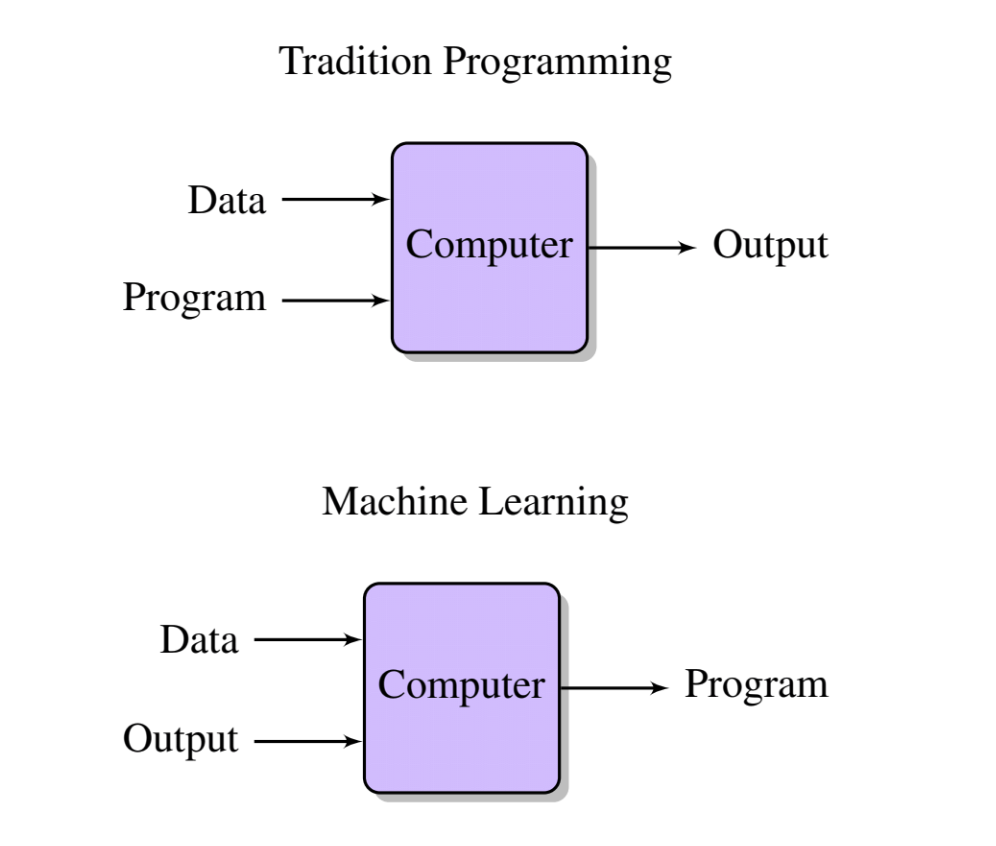
\includegraphics[width=0.8 \linewidth]{images/ml.png}
    \caption{Difference between traditional computing and machine learning: while in the former a program is provided to the machine, in the latter the machine itself is able to synthesize it.}
    \label{fig:ml} \end{figure}

% On top of this, many modern algorithms, such as Neural Networks, Ant Colony Optimization, Genetic Algorithms etc., have introduced some kind of non-determinism, which means that slightly different starting points may lead to very different solutions. These algorithms have proved to be very effective and can be applied to many problems, especially those that do not require an optimal solution, since they can explore a huge solution space until the solution is ``good enough''.

Randomness and learning cause the developer of an AI algorithm to not be fully in control of all the decisions that the AI system makes, which motivates the idea that AI behaves as a \textit{black box}.


\subsection{Explaining AI: a toy example}
\label{sec:example}

As an example of the problem of explaining an AI system, we can take a look to what it is like to work on a Neural Network. A conceptual representation of a
Neural Network's structure is depicted in Figure~\ref{fig:nn}.

\begin{figure}[ht!] \centering 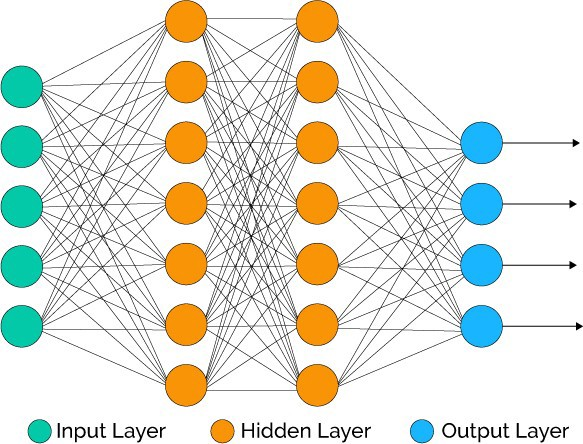
\includegraphics[width=0.8 \linewidth]{images/nn}
    \caption{Conceptual representation of the layers of an Artificial Neural Network}
    \label{fig:nn} \end{figure}

This graphical representation is useful for understanding the general
architecture of the algorithm, but it doesn't really tell us anything about
how the Neural Network actually works, i.e. what is the relationship between a
certain input and its output.

We could give a more precise representation of this dependency in
Figure~\ref{fig:mathnn}, which explicitly defines the mathematical relationship
between the input and the output. Although being more precise, we can see how we would still have a hard time
understanding what a Neural Network does if we were to adopt this
representation, especially in Deep Neural Networks with lots of intermediate layers between the input and the output.

\begin{figure}[ht!] \centering
    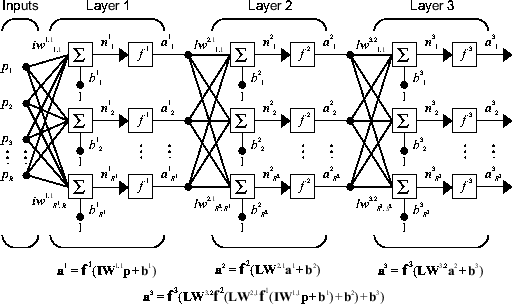
\includegraphics[width=0.9\linewidth]{images/nmodel} \caption{Mathematical
        equivalent representation} \label{fig:mathnn} \end{figure}

% As a counterexample, Figure~\ref{fig:dectree} represents a \textit{Decision Tree},
% another family of AI algorithms.


% There is a clear difference with the previous example: by looking at the structure of the algorithm we can immediately be sure of what decisions it is going to take, and get a grasp on the chain of reasons that caused a specific output. The main issue of these algorithms is that, for complex problems, they tend to be outperformed by Neural Networks, and the efficient variations of these techniques such as Random Forest greatly increase the complexity of the decision trees, which can grow very big and hence be very hard to understand.

This simple example shows how the solution space to the explainability problem
has multiple dimensions, constraints and trade-offs that have to be taken into
account.

\subsection{Bias problems in AI}
\label{sec:bias}

The problem of hidden bias in AI is a well-known issue of current AI.

\todo[inline]{Data bias in AI, demonstrate how vulnerable is AI to biases}

% \subsection{AI failures}
% \label{sec:aifails}

% First of all, the
% concept of complexity is different among humans and AIs: what might be simple
% for a human can be an extremely difficult task for an AI, such as image
% recognition, natural language processing and coming up with creative ideas. This
% creates a situation in which even AIs that are able to solve incredibly complex
% problems will occasionally fail in situations in which a human would have no
% problem at finding the correct solution. This happens for example in facial
% recognition, where most systems can be fooled by simply coloring the person's
% face in a certain way, or by hiding a specific portion of the face that for some
% reason happens to be important for the AI algorithm. \cit

% Another problem that has been found to affect many AI systems based on Machine
% Learning is that biased data will generate biased AI models. A famous example of
% this is the COMPAS algorithm, an algorithm used in US court systems to predict
% the likelihood that a defendant would become recidivist: due to the data that
% was used, the model predicted twice as many false positives for recidivism for
% black offenders (45\%) than white offenders (23\%). \cit Similarly, in 2015
% Amazon realized that their algorithm used for hiring employees was biased
% against women: because the algorithm was based on the number of resumes
% submitted over the past ten years, and since most of the applicants were men, it
% was trained to favor men over women. \cit The problem of debiasing AIs is still
% an open problem today, and there is no simple solution to it. \cit

% Finally, AI systems are unpredictable and obscure, even to those who develop
% them: an AI can seem to behave very well on a given test set, and yet suddenly
% break or have behave strangely when deployed in the real-world. This happens for example in ``Clever Hans'' situations, a well-known problem of AI, in which an AI might associate the outcome of a problem with an element of the input that in reality is totally unrelated from the pattern that needs to be identified, e.g. an AI system that recognizes the content of a photo based on the copyright notice at the end of it instead of looking to the real content. \cit

% \todo[inline]{flash crash}

% It is important to notice that the problems highlighted in the above examples
% cannot be associated to any particular module or feature of the AI system itself: there is
% no such thing as ``fixing one line of code'' for these systems.

%-----------------------------------------------------------------%
\section{The XAI approach}
\label{sec:xai}

\subsection{Goals}

Explainable AI is a new research line that was proposed by
DARPA \cit, the same agency where the term "Artificial Intelligence" was born in
the first place \cit, in \todo[inline, inlinewidth=1.cm, noinlinepar]{anno}. It
is meant to be give birth to a new generation of Artificial Intelligence systems which are
designed to be easier to understand by humans. In particular, the goal of XAI is
to make Artificial Intelligence more:

\begin{itemize}
    \item \textit{Easy to debug }for the developers
    \item \textit{Predictable}, so that companies and governments adopting this
          technology can be aware of the possible weaknesses
    \item \textit{Trustful} for operators and end-users of this technology
\end{itemize}

Figure~\ref{fig:xai} describes the end result that is expected from XAI.


\begin{figure}[h!] 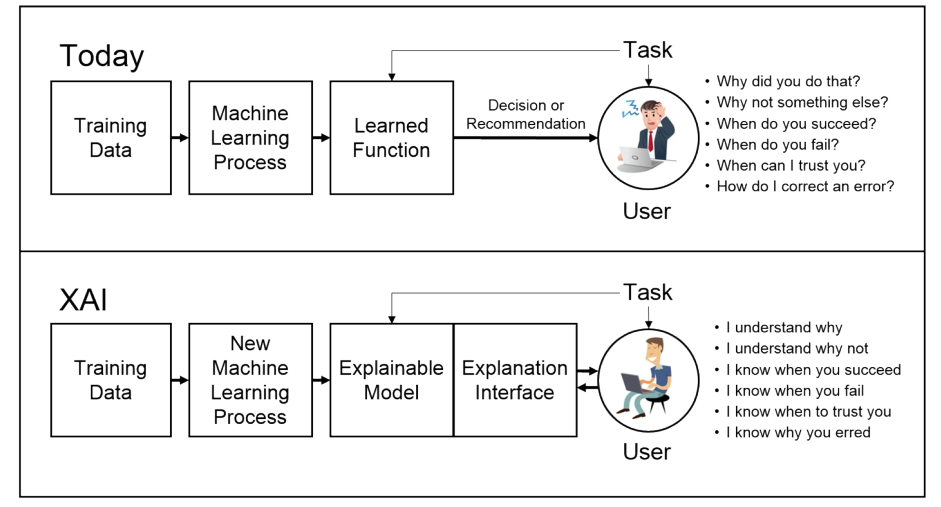
\includegraphics[width=\linewidth]{images/xai.png}
    \caption{The goal of XAI as expressed in the official DARPA presentation of the XAI project. \todo[inline]{cit}} \label{fig:xai} \end{figure}

The creation of XAI requires the join effort in a variety of research fields,
from Computer Science to Cognitive Psychology, and there is still a lot of work
to do. Nevertheless already many papers have been submitted on the subject,
indicating a growing interest of the research community towards this subject.

\subsection{Current Solutions}
\label{sec:solutions}

Given the highly experimental nature of this topic, many different solutions
have been proposed by various papers in the framework of XAI, which vary greatly
in intended use, goal and adopted approach. \cit contains a classification of the existing XAI
solutions and their respective strengths and weaknesses, which are classified as shown in Figure~\ref{fig:xaiclass}.

\begin{figure}[h!] 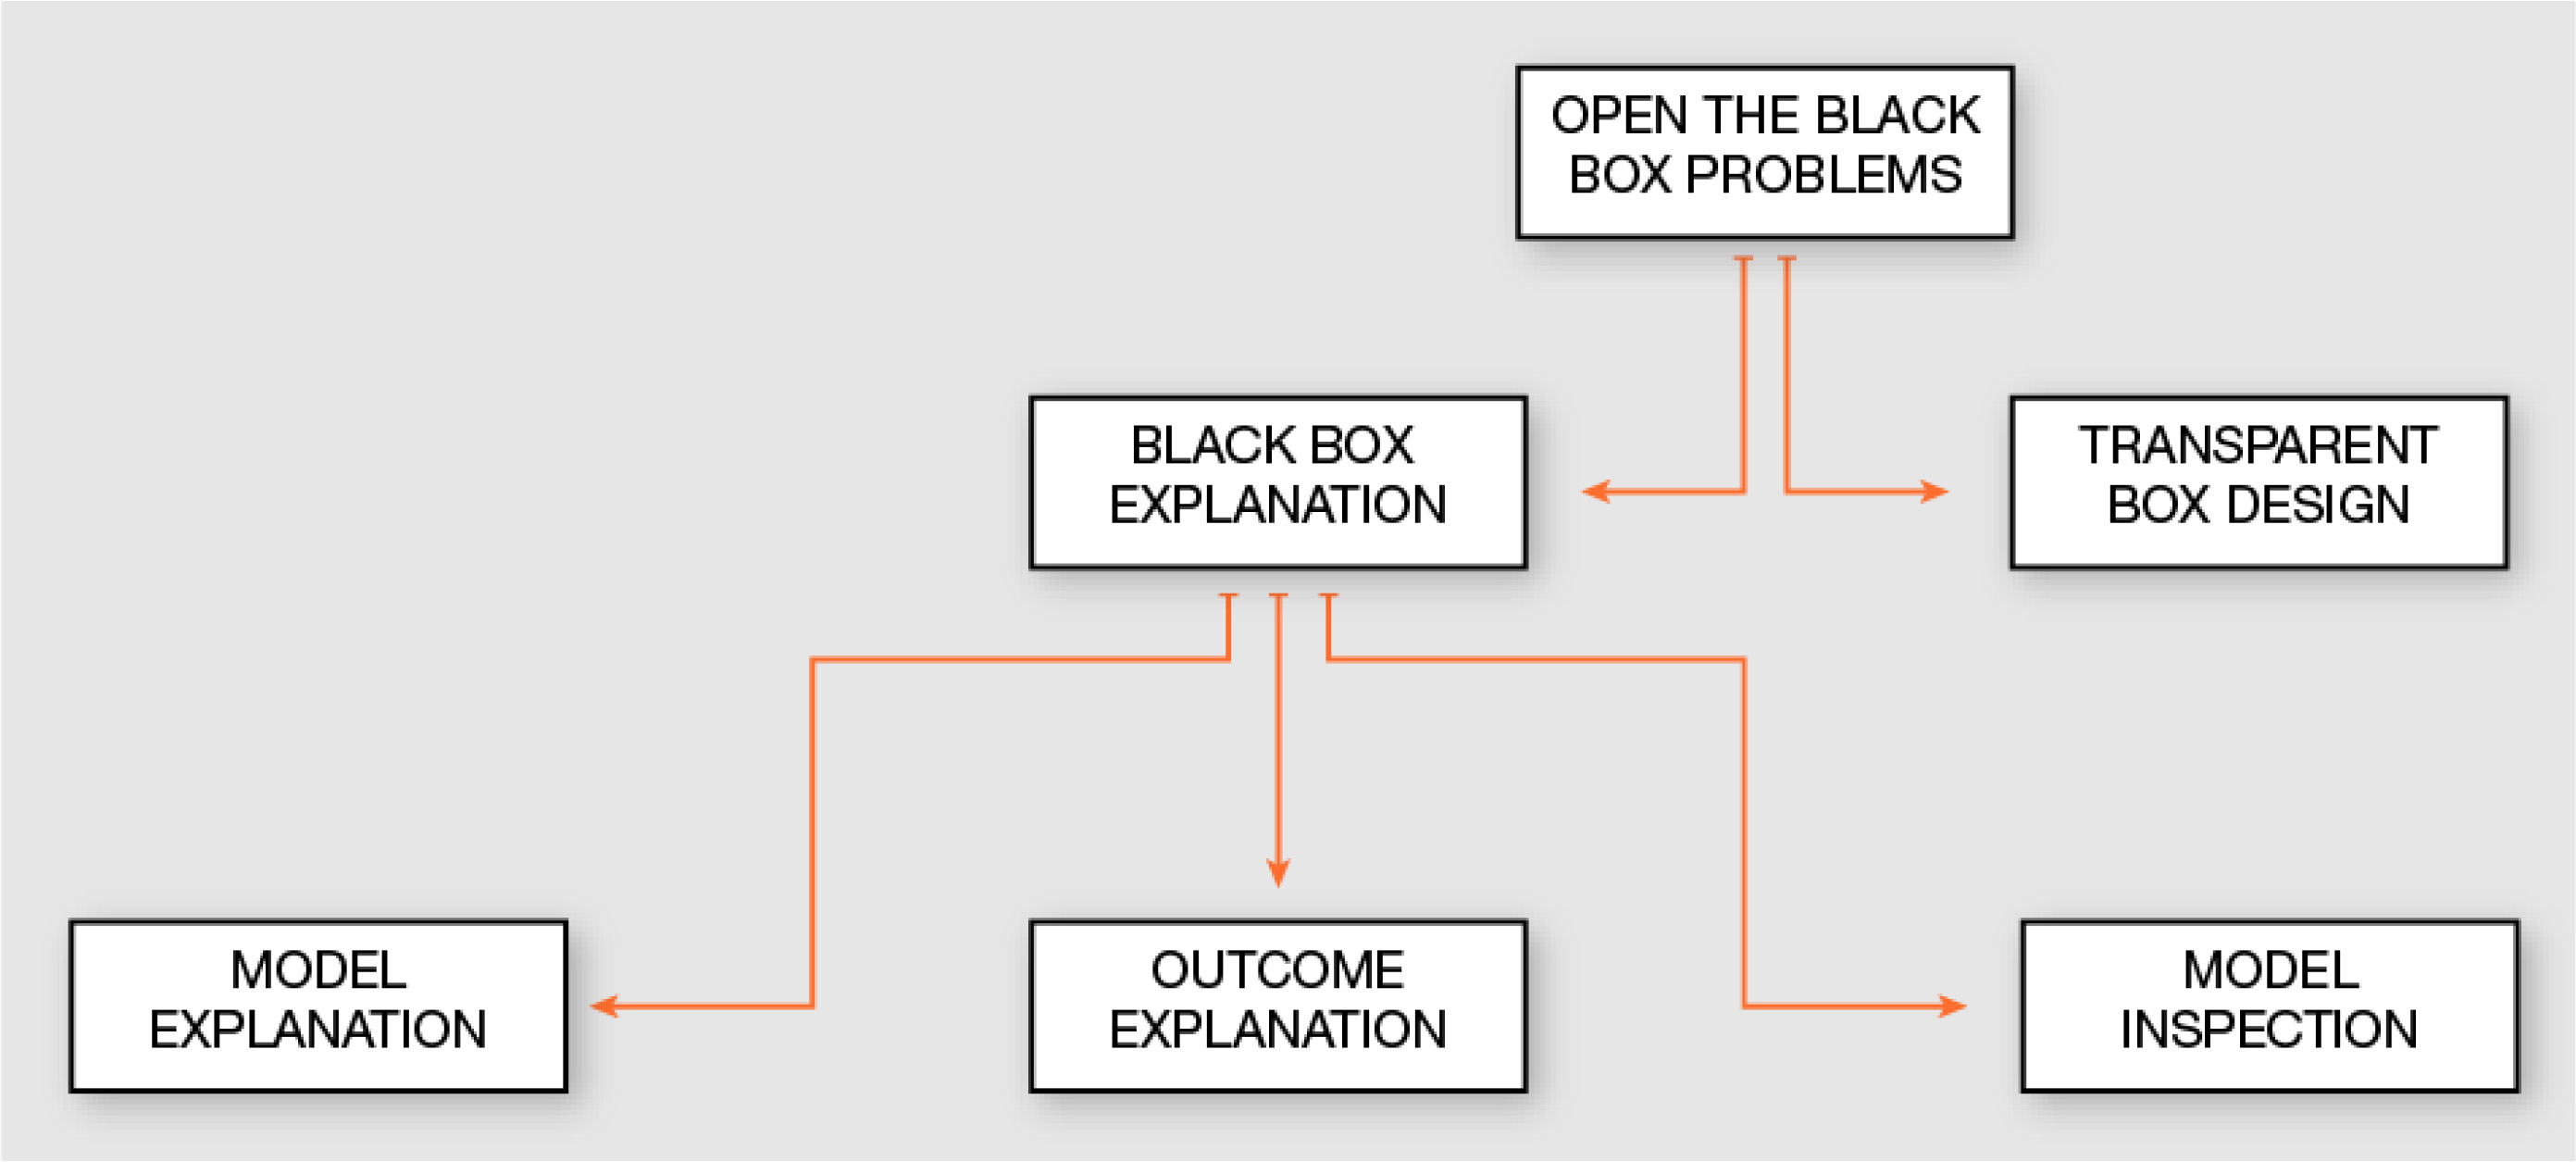
\includegraphics[width=\linewidth]{images/xaiclass.png}
    \caption{Taxonomy of XAI solutions provided by \todo[inline]{cit}} \label{fig:xaiclass} \end{figure}

The main techniques identified are:
\begin{itemize}
    \item \textit{Model explanation}: Global explanation of the whole model's behavior.
    \item \textit{Outcome explanation}: Local explanation of a single outcome.
    \item \textit{Model inspection}: Explanation trough introspection of the model's internals.
    \item \textit{Transparent Box design}: Making AI easier to understand by design, e.g. by using algorithms that are intrinsically clearer for humans.
\end{itemize}

With no aim of being
exhaustive, we want to provide an abstract
classification of the main XAI solutions, based their general approach to the
problem.

XAI approaches might be classified as:

\begin{enumerate}
    \item \textbf{Visualization}: these approaches focus on finding an effective
          way representation to visually represent key aspects of the AI
          behavior. One example is to use \textit{saliency masks}, such as the
          one in Figure~\ref{fig:heatmap}, to highlight which are the most
          significant portions of the input for the AI model, or in general to
          visually express which are the most important features that the model is recognizing. This is generally good for applications which are based on images, but might not be enough in other situations.

          \begin{figure}[h!] 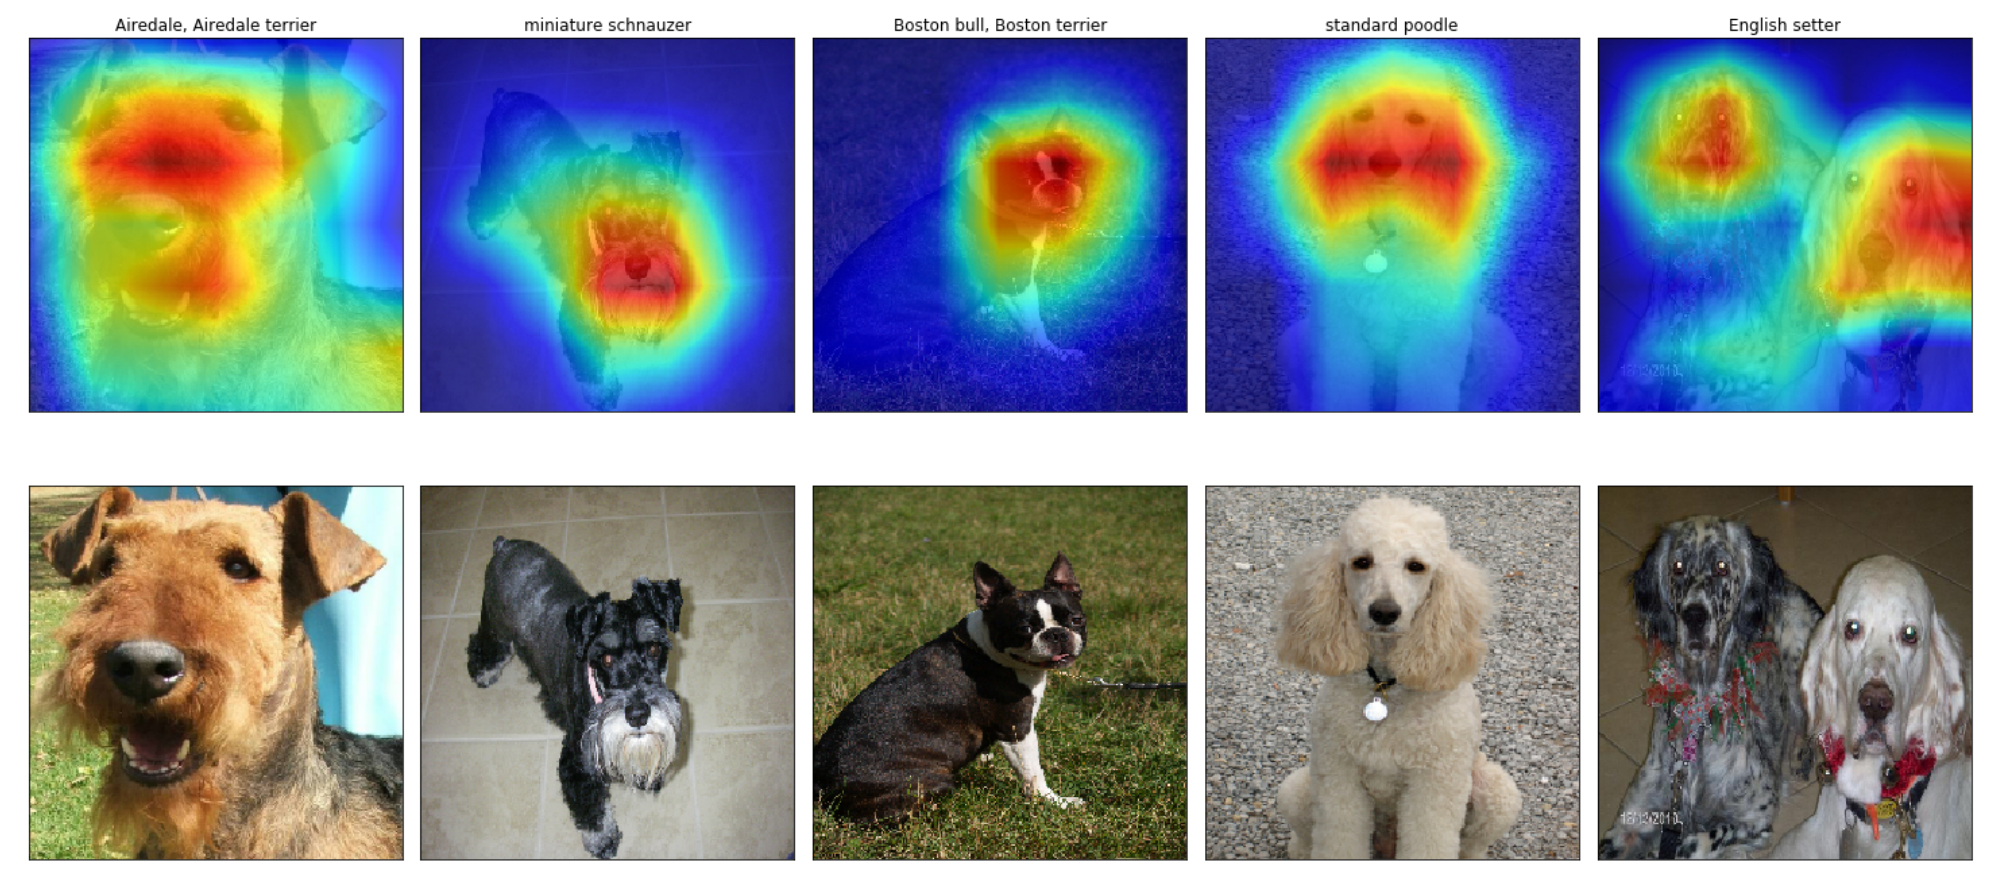
\includegraphics[width=\linewidth]{images/dog_localization.png}
              \caption{An example of a heatmap representing the importance of pixels in a given picture, from blue (low importance) to red (high importance). \todo[inline]{cit}} \label{fig:heatmap} \end{figure}

    \item \textbf{Approximation}: this approach consists in trying to adopt
          models that are simpler by design, or simplifying already existing models to just a set of important features. This is the case of \textit{single tree approximation} \cit, where the internal structure of an AI algorithm is approximated to a singe classification tree, such as in Figure~\ref{fig:dectree}.

          \begin{figure}[ht!] \centering
              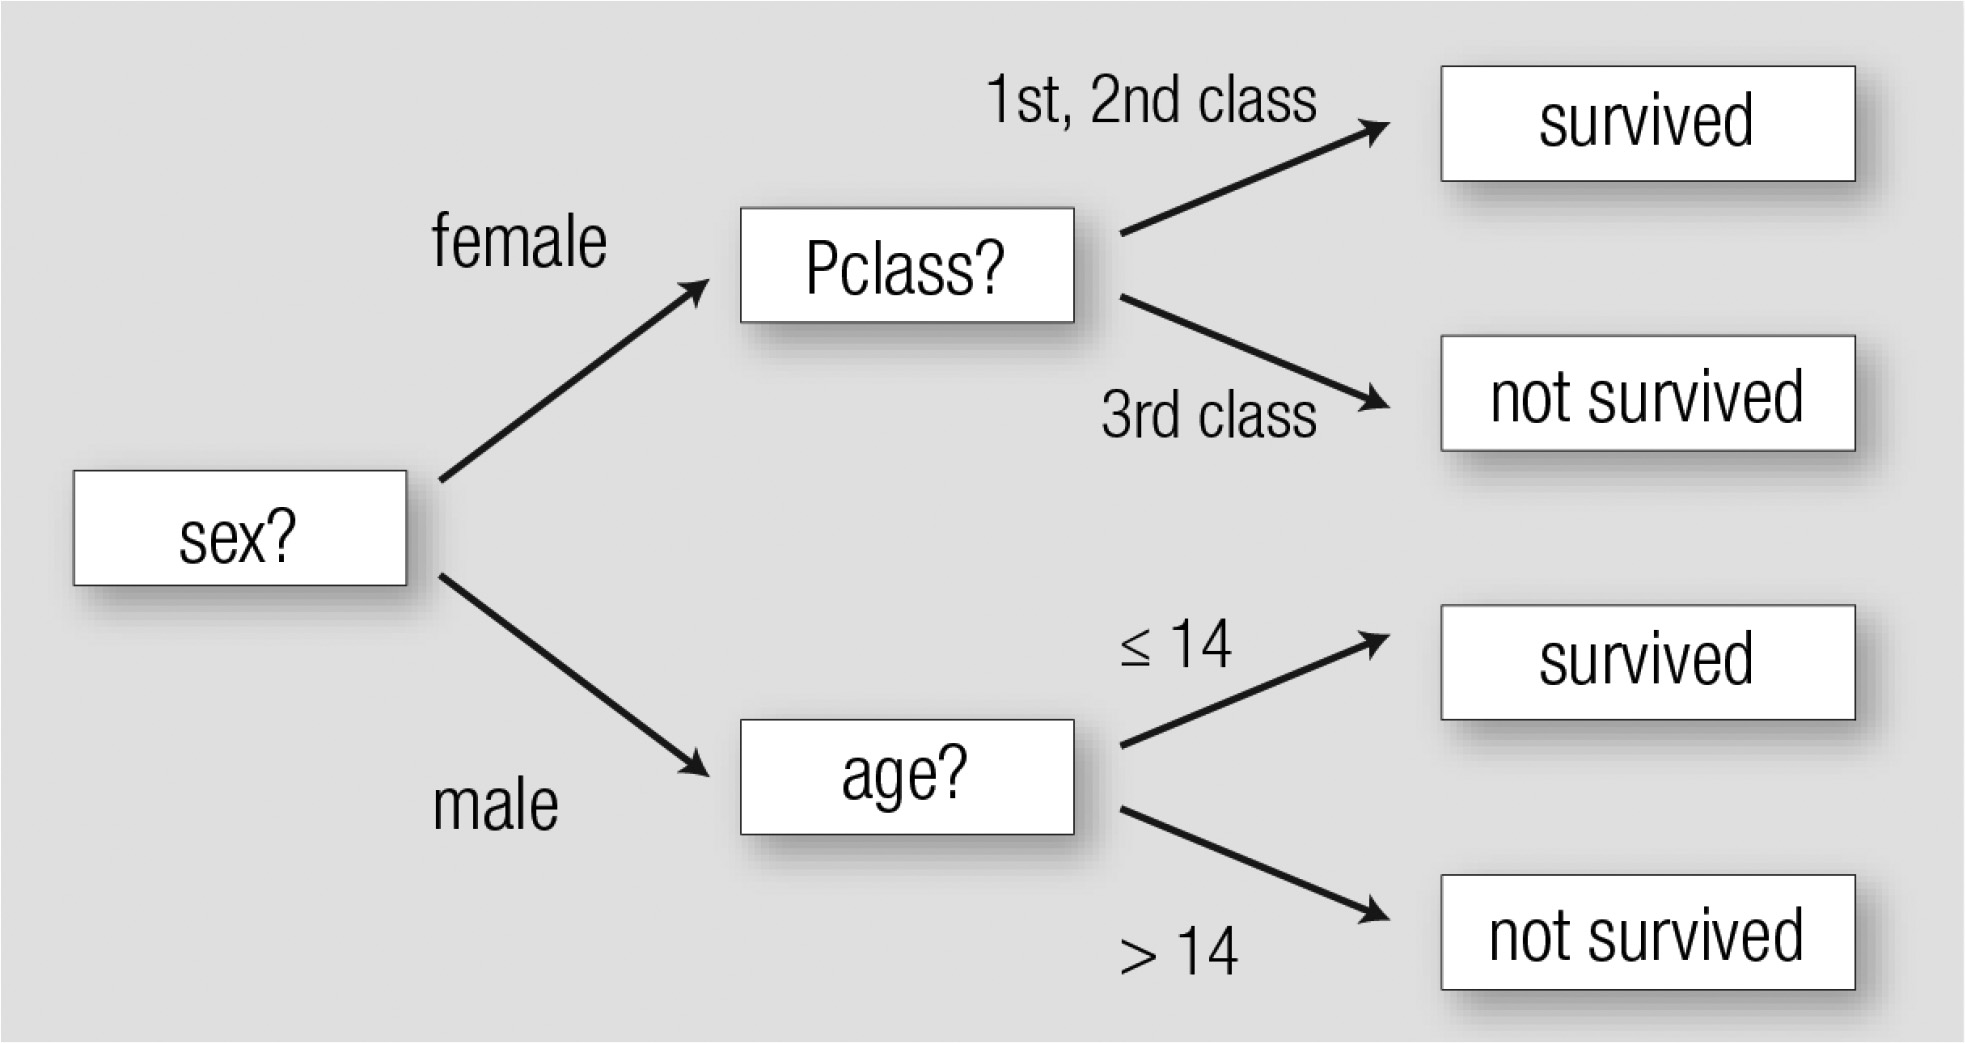
\includegraphics[width=0.9\linewidth]{images/dectree} \caption{A simple
                  Decision Tree} \label{fig:dectree} \end{figure}

    \item \textbf{Behavioral Model}: this explanation technique focuses on expressing the dependencies
          between inputs and outputs ignoring the internal structure. This means, in
          practice, creating a behavioral model of the algorithm which is
          parallel to the algorithm itself, and can be expressed in an easier form, such as a set of logical rules.
    \item \textbf{Explanation by Example}: a nice information to have when
          trying to understand an AI model, especially in the case of
          classifiers, is an example, or a \textit{prototype}, of how the AI
          thinks that a typical member of a given class should appear. This can
          be realized in many ways, for example by attaching to a classification
          output a set of minimal changes to the input that would cause the
          output to be modified, or specify a partially filled object for each
          class.
\end{enumerate}

%-----------------------------------------------------------------%
\section{Defining Explainability}
\label{sec:explainability}

As we anticipated in Section~\ref{sec:intro}, one fundamental problem in
the field of XAI is that there is no single conventional notion of
explainability.

If, on one hand, many solutions have already been proposed to tackle the
problem, with various claims regarding their interpretability, on the other hand
the lack of a formal definition seriously challenges the findings of these
researches, casting a shade of doubt on the proposed solutions.

Mythos\cit goes as far as considering the term itself ill-defined, therefore
stating that claims about interpretability generally have a quasi-scientific
nature. Giannotti\cit on the other hand, in a review of the current state of the
art, considers the lack of a mathematical description as an obstacle for the
future development of this field. The DARPA paper \cit itself defines the
formalization of an evaluation metric for explanations as one of the goals of
the XAI project, to be developed in parallel with technical solutions.

Without discouraging the research on this matter, we want to highlight that this
is easier said than done.

\subsection{What is the scope?}

Before evaluating an explanation interface or an XAI system in general, we
should ask ourselves at least the following questions:

\

\textbf{Explainable to whom?} The concept of \textit{user} of an AI system is
not always well defined, nor is the concept of user of an explanation. This
might include:

\begin{itemize}
    \item The \textbf{developer} of the AI system, as he is only partially in
          control of what the algorithm does (refer to Section~\ref{sec:aiprog})
    \item The \textbf{operator} of an AI system: many AI algorithms nowadays are
          being used as an input for a human to make decisions on a certain
          subject
    \item The \textbf{end user} which is affected by the decision of an AI
\end{itemize}

\

\textbf{Explainable for which purpose?} Different users have different needs,
that can partially overlap, when it comes to AI explanation. More in general,
whether a certain representation can be considered explanatory depends to some
degree on what it is being used for. In the case of XAI, some common purposes
are:

\begin{itemize}
    \item \textbf{Debugging}: finding errors or underperforming portions of the
          system
    \item \textbf{Human-in-the-loop}: creating systems where human and AI
          decisions can co-exist and influence each other
    \item \textbf{Validation}: understanding if a certain model is good enough
          to be deployed for a certain tasks, where it fails and what happens
          when it fails
    \item \textbf{Appeal AI decisions}: \footnote{This last goal is not
              explicitly listed in the original scope of XAI goals, but has
              gained traction recently with the publication of \textit{right for
                  an explanation} law in EU. \todo[inline]{cit}} giving the right to
          users and citizens that are affected by AI decisions to know,
          understand and possibly appeal decisions that are automated with
          AI systems
\end{itemize}

\

It appears quite evident that different XAI solutions with different scopes and
intended users cannot be compared in the same way.

\subsection{Possible Metrics}
\label{sec:dimensions}

Bearing in mind the different goals that an XAI system can have, we can identify
a series of characteristics that are different among different solutions:

\begin{itemize}
    \item \textbf{Complexity}: how many elements are there in the explanation?
    \item \textbf{Clearness}: how cognitively hard is the explanation? How
          difficult is it to understand the correspondence between the elements
          of the explanation and the information we are trying to gain?
    \item \textbf{Informativeness}: how much information, weighted on how
          meaningful is is, can be extracted by the explanation? E.g. does the
          explanation significantly modify the level of uncertainty about the AI
          behavior?
    \item \textbf{Fidelity}: how closely does the explanation represent the
          internal functioning of the system? Are all the facts inferred from
          the explanation also applicable to the original system?
\end{itemize}

Clearly, the choice of the evaluation metric.

%-----------------------------------------------------------------%
\section{The troubles of explanations}
\label{sec:troubles}

\subsection{Measuring fidelity}
\label{sec:fidelity}

\subsection{Fidelity vs Complexity tradeoff}
\label{sec:tradeoff}

\subsection{How can an explanation introduce bias?}
\label{sec:bias}


%-----------------------------------------------------------------%
\section{Conclusions}
\label{sec:conclusions}

In conclusion, the main problem of XAI is that there is no single definition of
what an explanation is, it depends on the purpose and on the user of the AI
system.

For this reason, these should be considered different problems, at least the
debugging problem vs the right of explanation problem: they are not correlated
and saying that one solves the other poses some threats on the quality of the
result itself.

``I always thought something was fundamentally wrong with the universe''

\citep{adams1995hitchhiker}

\bibliographystyle{plain}
\bibliography{references}
\end{document}
